\documentclass[tikz]{standalone}
\usepackage[charter]{mathdesign}

\usetikzlibrary{arrows, arrows.meta, matrix}
\tikzset{headarrow/.style = {-{Latex[length=.5em]}}}

\begin{document}
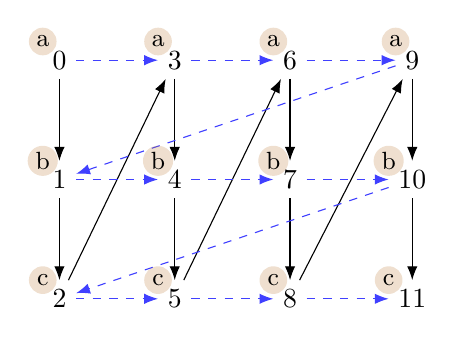
\begin{tikzpicture}
    \node (m) at (0,0) [matrix of nodes,
                        row sep=3em, column sep=3em] {%
    0 & 3 & 6 & 9\\
    1 & 4 & 7 & 10\\
    2 & 5 & 8 & 11\\
    };

    \foreach \Target [remember=\Target as \Source (initially 1-1)] in {%
        2-1,
        3-1,
        1-2,
        2-2,
        3-2,
        1-3,
        2-3,
        3-3,
        1-4,
        2-4,
        3-4%
        }
        \draw[headarrow] (m-\Source) to (m-\Target);

    \foreach \Target [remember=\Target as \Source (initially 1-1)] in {%
        1-2,
        1-3,
        1-4,
        2-1,
        2-2,
        2-3,
        2-4,
        3-1,
        3-2,
        3-3,
        3-4%
        }
        \draw[headarrow, dashed, blue!75] (m-\Source) to (m-\Target);

    \foreach \y in {1,...,4}
        \foreach \x/\Label in {%
            1/a,
            2/b,
            3/c%
            }
            \node[circle,
                  fill=brown, fill opacity=.25,
                  inner sep=.1em, minimum size=1em] at
                  (m-\x-\y.north west) [font=\small, text opacity=1] {\Label};
\end{tikzpicture}
\end{document}
